\hypertarget{dcel---doubly-connected-edge-list}{%
\section{DCEL - Doubly Connected Edge
List}\label{dcel---doubly-connected-edge-list}}

\hypertarget{introduction}{%
\subsection{Introduction}\label{introduction}}

Doubly connected edge list (DCEL), which is also known as halfedge data
structure, is used to efficiently represent planar graphs. Using a DCEL
structure, we can easily manipulate the topological information of the
planar graph such as vertices, faces and edges.

In general, a DCEL conatins a book-keeping record of all edges, vertices
and faces of the graph. Each record individually can contain information
of all it's incident geometric objects. We will look at how a DCEL
stores this information in
\protect\hyperlink{data-structure-approach}{Data Structure Approach}
section.

\hypertarget{how-to-run}{%
\subsection{How to Run}\label{how-to-run}}

The src folder contains the source code for the DCEL data structure.
\texttt{g++} from the GNU compiler suite is required to compile the
program to a executable.

Steps to Compile:

\begin{enumerate}
\def\labelenumi{\arabic{enumi})}
\tightlist
\item
  \texttt{cd} into the src directory
\item
  Run \texttt{g++\ main.cpp} which generates an executable called
  \texttt{a.out} in the same directory
\item
  Run the executable using \texttt{./a.out} (on linux)

  \begin{enumerate}
  \def\labelenumii{\arabic{enumii})}
  \tightlist
  \item
    The executable takes a dataset from command line argument. For
    example, to use an existing dataset, run
    \texttt{./a.out\ ../datasets/1sq.txt}
  \item
    If no command-line argument is given, it takes input from the shell
    directly (stdin)
  \end{enumerate}
\end{enumerate}

\hypertarget{input}{%
\subsection{Input}\label{input}}

The required input format for the algorithm to work correctly is:

\begin{itemize}
\tightlist
\item
  Input can be given both from file (via command-line args) or stdin
\item
  First line must contain the no of Edges to be taken as input by the
  program.
\item
  Each of next line must contain 4 integers, space seperated denoting
  the (x1, y1), (x2, y2) coordinates of endpoints of each edge.
\item
  Each coordinate must be of integer type in the range -10\^{}8 to
  10\^{}8.
\item
  Number of coordinates must be less than 1 Billion.
\end{itemize}

\hypertarget{output}{%
\subsection{Output}\label{output}}

Output of the algorithm prints all the HalfEdges incident to each face
by traversing its representative half edges. All the faces outputed by
the program can also be verified by running it through the plotting
diagram.\\
The last two lines of output show the time taken to take input in
microseconds and the time taken by the algorithm to compute DCEL (also
in microseconds).

An example of output of dataset
\href{./datasets/random4.txt}{random4.txt}:

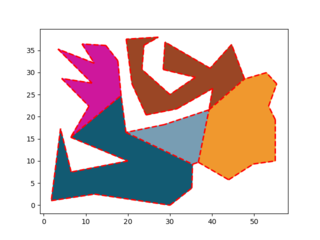
\includegraphics[width=8cm,height=8cm]{img/DCELrandom.png}\\

\hypertarget{documentation-and-report}{%
\subsection{Documentation and Report}\label{documentation-and-report}}

Documentation of this algorithm, functions and classes can be found in
the \texttt{docs} folder in the current directory. Open the
\href{../DCEL/docs/html/index.html}{index.html} file from the docs
directory with your preferred browser to go through the documentation

\hypertarget{performance-analysis}{%
\subsection{Performance Analysis}\label{performance-analysis}}

This analysis does not include the time taken to show output on
terminal. Analysis is performed with a system running:

\begin{itemize}
\tightlist
\item
  OS: Arch Linux (64Bit) running Linux Kernel version 5.7.2
\item
  Processor: Intel Core i7 7700HQ
\item
  RAM: 8GB
\item
  Compiler: GNU G++ (GCC) 10.1.0
\end{itemize}

\textbf{The following observations are recorded:}

Manual generated test files:

\begin{longtable}[]{@{}lccccc@{}}
\toprule
\begin{minipage}[b]{0.12\columnwidth}\raggedright
Filename\strut
\end{minipage} & \begin{minipage}[b]{0.15\columnwidth}\centering
Input Vertices\strut
\end{minipage} & \begin{minipage}[b]{0.12\columnwidth}\centering
Input Edges\strut
\end{minipage} & \begin{minipage}[b]{0.12\columnwidth}\centering
Input Faces\strut
\end{minipage} & \begin{minipage}[b]{0.15\columnwidth}\centering
File read time\strut
\end{minipage} & \begin{minipage}[b]{0.17\columnwidth}\centering
DCEL Creation Time\strut
\end{minipage}\tabularnewline
\midrule
\endhead
\begin{minipage}[t]{0.12\columnwidth}\raggedright
1sq.txt\strut
\end{minipage} & \begin{minipage}[t]{0.15\columnwidth}\centering
4\strut
\end{minipage} & \begin{minipage}[t]{0.12\columnwidth}\centering
4\strut
\end{minipage} & \begin{minipage}[t]{0.12\columnwidth}\centering
2\strut
\end{minipage} & \begin{minipage}[t]{0.15\columnwidth}\centering
505 microsec\strut
\end{minipage} & \begin{minipage}[t]{0.17\columnwidth}\centering
27 microsec\strut
\end{minipage}\tabularnewline
\begin{minipage}[t]{0.12\columnwidth}\raggedright
4sq.txt\strut
\end{minipage} & \begin{minipage}[t]{0.15\columnwidth}\centering
9\strut
\end{minipage} & \begin{minipage}[t]{0.12\columnwidth}\centering
12\strut
\end{minipage} & \begin{minipage}[t]{0.12\columnwidth}\centering
5\strut
\end{minipage} & \begin{minipage}[t]{0.15\columnwidth}\centering
396 microsec\strut
\end{minipage} & \begin{minipage}[t]{0.17\columnwidth}\centering
46 microsec\strut
\end{minipage}\tabularnewline
\begin{minipage}[t]{0.12\columnwidth}\raggedright
random1.txt\strut
\end{minipage} & \begin{minipage}[t]{0.15\columnwidth}\centering
10\strut
\end{minipage} & \begin{minipage}[t]{0.12\columnwidth}\centering
12\strut
\end{minipage} & \begin{minipage}[t]{0.12\columnwidth}\centering
4\strut
\end{minipage} & \begin{minipage}[t]{0.15\columnwidth}\centering
257 microsec\strut
\end{minipage} & \begin{minipage}[t]{0.17\columnwidth}\centering
52 microsec\strut
\end{minipage}\tabularnewline
\begin{minipage}[t]{0.12\columnwidth}\raggedright
random3.txt\strut
\end{minipage} & \begin{minipage}[t]{0.15\columnwidth}\centering
23\strut
\end{minipage} & \begin{minipage}[t]{0.12\columnwidth}\centering
26\strut
\end{minipage} & \begin{minipage}[t]{0.12\columnwidth}\centering
5\strut
\end{minipage} & \begin{minipage}[t]{0.15\columnwidth}\centering
175 microsec\strut
\end{minipage} & \begin{minipage}[t]{0.17\columnwidth}\centering
84 microsec\strut
\end{minipage}\tabularnewline
\begin{minipage}[t]{0.12\columnwidth}\raggedright
random2.txt\strut
\end{minipage} & \begin{minipage}[t]{0.15\columnwidth}\centering
23\strut
\end{minipage} & \begin{minipage}[t]{0.12\columnwidth}\centering
37\strut
\end{minipage} & \begin{minipage}[t]{0.12\columnwidth}\centering
16\strut
\end{minipage} & \begin{minipage}[t]{0.15\columnwidth}\centering
192 microsec\strut
\end{minipage} & \begin{minipage}[t]{0.17\columnwidth}\centering
102 microsec\strut
\end{minipage}\tabularnewline
\begin{minipage}[t]{0.12\columnwidth}\raggedright
a.txt\strut
\end{minipage} & \begin{minipage}[t]{0.15\columnwidth}\centering
31\strut
\end{minipage} & \begin{minipage}[t]{0.12\columnwidth}\centering
33\strut
\end{minipage} & \begin{minipage}[t]{0.12\columnwidth}\centering
4\strut
\end{minipage} & \begin{minipage}[t]{0.15\columnwidth}\centering
150 microsec\strut
\end{minipage} & \begin{minipage}[t]{0.17\columnwidth}\centering
109 microsec\strut
\end{minipage}\tabularnewline
\begin{minipage}[t]{0.12\columnwidth}\raggedright
random4.txt\strut
\end{minipage} & \begin{minipage}[t]{0.15\columnwidth}\centering
44\strut
\end{minipage} & \begin{minipage}[t]{0.12\columnwidth}\centering
48\strut
\end{minipage} & \begin{minipage}[t]{0.12\columnwidth}\centering
6\strut
\end{minipage} & \begin{minipage}[t]{0.15\columnwidth}\centering
364 microsec\strut
\end{minipage} & \begin{minipage}[t]{0.17\columnwidth}\centering
165 microsec\strut
\end{minipage}\tabularnewline
\begin{minipage}[t]{0.12\columnwidth}\raggedright
house.txt\strut
\end{minipage} & \begin{minipage}[t]{0.15\columnwidth}\centering
71\strut
\end{minipage} & \begin{minipage}[t]{0.12\columnwidth}\centering
81\strut
\end{minipage} & \begin{minipage}[t]{0.12\columnwidth}\centering
12\strut
\end{minipage} & \begin{minipage}[t]{0.15\columnwidth}\centering
250 microsec\strut
\end{minipage} & \begin{minipage}[t]{0.17\columnwidth}\centering
300 microsec\strut
\end{minipage}\tabularnewline
\bottomrule
\end{longtable}

Using real world datasets:

\begin{itemize}
\tightlist
\item
  Road network of hyderabad, source: GPS coordinates filtered from
  osm(openstreetmap) data on hyderabad

  \begin{itemize}
  \tightlist
  \item
    hyd\_1.txt: contains road network having tag of \emph{highway} set
    as `trunk'
  \item
    hyd\_2.txt: contains road network having tag of \emph{highway} set
    as `trunk' and `primary'
  \item
    hyd\_2.txt: contains road network having tag of \emph{highway} set
    as `trunk', `primary' and `secondary'
  \item
    hyd\_2.txt: contains road network having tag of \emph{highway} set
    as `trunk', `primary', `secondary', and `motorway'
  \end{itemize}
\end{itemize}

\begin{longtable}[]{@{}lccccc@{}}
\toprule
\begin{minipage}[b]{0.12\columnwidth}\raggedright
Filename\strut
\end{minipage} & \begin{minipage}[b]{0.15\columnwidth}\centering
Input Vertices\strut
\end{minipage} & \begin{minipage}[b]{0.12\columnwidth}\centering
Input Edges\strut
\end{minipage} & \begin{minipage}[b]{0.12\columnwidth}\centering
Input Faces\strut
\end{minipage} & \begin{minipage}[b]{0.15\columnwidth}\centering
File read time\strut
\end{minipage} & \begin{minipage}[b]{0.17\columnwidth}\centering
Algorithm runtime\strut
\end{minipage}\tabularnewline
\midrule
\endhead
\begin{minipage}[t]{0.12\columnwidth}\raggedright
hyd\_1.txt\strut
\end{minipage} & \begin{minipage}[t]{0.15\columnwidth}\centering
685\strut
\end{minipage} & \begin{minipage}[t]{0.12\columnwidth}\centering
733\strut
\end{minipage} & \begin{minipage}[t]{0.12\columnwidth}\centering
58\strut
\end{minipage} & \begin{minipage}[t]{0.15\columnwidth}\centering
2.4 millisec\strut
\end{minipage} & \begin{minipage}[t]{0.17\columnwidth}\centering
1.68 millisec\strut
\end{minipage}\tabularnewline
\begin{minipage}[t]{0.12\columnwidth}\raggedright
hyd\_2.txt\strut
\end{minipage} & \begin{minipage}[t]{0.15\columnwidth}\centering
1787\strut
\end{minipage} & \begin{minipage}[t]{0.12\columnwidth}\centering
1912\strut
\end{minipage} & \begin{minipage}[t]{0.12\columnwidth}\centering
229\strut
\end{minipage} & \begin{minipage}[t]{0.15\columnwidth}\centering
3.5 millisec\strut
\end{minipage} & \begin{minipage}[t]{0.17\columnwidth}\centering
107.5 millisec\strut
\end{minipage}\tabularnewline
\begin{minipage}[t]{0.12\columnwidth}\raggedright
hyd\_3.txt\strut
\end{minipage} & \begin{minipage}[t]{0.15\columnwidth}\centering
2959\strut
\end{minipage} & \begin{minipage}[t]{0.12\columnwidth}\centering
3198\strut
\end{minipage} & \begin{minipage}[t]{0.12\columnwidth}\centering
519\strut
\end{minipage} & \begin{minipage}[t]{0.15\columnwidth}\centering
5.4 millisec\strut
\end{minipage} & \begin{minipage}[t]{0.17\columnwidth}\centering
276.9 millisec\strut
\end{minipage}\tabularnewline
\begin{minipage}[t]{0.12\columnwidth}\raggedright
hyd\_4.txt\strut
\end{minipage} & \begin{minipage}[t]{0.15\columnwidth}\centering
3612\strut
\end{minipage} & \begin{minipage}[t]{0.12\columnwidth}\centering
3850\strut
\end{minipage} & \begin{minipage}[t]{0.12\columnwidth}\centering
532\strut
\end{minipage} & \begin{minipage}[t]{0.15\columnwidth}\centering
24.3 millisec\strut
\end{minipage} & \begin{minipage}[t]{0.17\columnwidth}\centering
337.8 millisec\strut
\end{minipage}\tabularnewline
\bottomrule
\end{longtable}

\hypertarget{data-structure-approach}{%
\subsection{Data Structure Approach}\label{data-structure-approach}}

The following geometric objects are used in DCEL:

\begin{itemize}
\tightlist
\item
  \textbf{Vertex}: Object to store vertex coordinates and any one of its
  incident halfedges as its representative.
\item
  \textbf{Edge}: Object to store its vertex endpoints.
\item
  \textbf{Face}: Object to store a unique face-id and one of its
  incident halfedges as its representative
\item
  \textbf{HalfEdge}: Object to store a directed halfedge which has
  pointers to all its incident geometric objects (Vertex, Face, next and
  previous halfedges and its twin halfedge)
\end{itemize}

This implementation uses a Hash Map to store list of all incident
halfedges for each vertex. This Hash Map uses vertex pointer as key and
stores a list of halfedges as value. Our DCEL also has a list of
Vertices and Faces which can be used to iterate through all Vertices and
Faces quickly.

A half-edge has a pointer to the next half-edge and previous half-edge
of the same face. Each half-edge has a single face as its representative
Face (which is present towards left side of it). All half-edges
associated with a face are counter-clockwise which can be obtained by
traversing its representative Halfedge. To reach the other face, we can
go to the twin of the half-edge and then traverse the other face. Each
half-edge also has a pointer to its origin vertex which can be used to
get all the Vertex points of the corresponding face.

\hypertarget{results}{%
\subsection{Results}\label{results}}

This algorithm to construct a DCEL takes time complexity of O(V+E). From
the analysis of example dataset runtimes, we can easily see that
increase in number of vertices and edges directly leads to increase in
DCEL construction time.

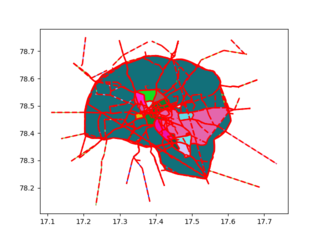
\includegraphics[width=8cm,height=8cm]{img/DCELhyd4.png}\\

The output of the algorithm is direct traversal of representative edges
of all faces present in the input. In the above example of Hyderabad
road network dataset, it shows all the faces bounded by the roads. All
faces might not be visible directly as the road system branches without
forming many faces. But as we zoom, the faces can be spotted between
roads.

\hypertarget{conclusion}{%
\subsection{Conclusion}\label{conclusion}}

The time complexity O(V+E) cannot be reduced further because to store
the graph, it is required to traverse through all Vertices and Edges
present in the graph. Although the current implementation only supports
connected graphs, it can also be extended to store disconnected
components using techniques like hidden vertices.

From the above results, we can be sure that DCEL can be a good candidate
data structure for easy representation of planar graphs. But as every
other data structure, even DCEL has it downfalls. The main one being the
amount of Storage required to store. The storage requirement can be
further reduced if we only need to store Vertices or Edges, but this
does not give huge improvements. Also, as the size of DCEL increases,
the time to add an extra edge increases in a linear fashion which might
be bad based on the application.DCEL is a simple data structure which
helps to easily manupulate the graph structre, but it might not be an
appropriate choice for low memory applications such as in embedded
systems.
